% Format teze zasnovan je na paketu memoir
% http://tug.ctan.org/macros/latex/contrib/memoir/memman.pdf ili
% http://texdoc.net/texmf-dist/doc/latex/memoir/memman.pdf
% 
% Prilikom zadavanja klase memoir, navedenim opcijama se podešava 
% veličina slova (12pt) i jednostrano štampanje (oneside).
% Ove parametre možete menjati samo ako pravite nezvanične verzije
% mastera za privatnu upotrebu (na primer, u b5 varijanti ima smisla 
% smanjiti 
\documentclass[12pt,oneside]{memoir}

% Paket koji definiše sve specifičnosti mastera Matematičkog fakulteta
\usepackage{matfmaster}
%
% Podrazumevano pismo je ćirilica.
%   Ako koristite pdflatex, a ne xetex, sav latinički tekst na srpskom jeziku
%   treba biti okružen sa \lat{...} ili \begin{latinica}...\end{latinica}.
%
% Opicija [latinica]:
%   ako želite da pišete latiniciom, dodajte opciju "latinica" tj.
%   prethodni paket uključite pomoću: \usepackage[latinica]{matfmaster}.
%   Ako koristite pdflatex, a ne xetex, sav ćirilički tekst treba biti
%   okružen sa \cir{...} ili \begin{cirilica}...\end{cirilica}.
%
% Opcija [biblatex]:
%   ako želite da koristite reference na više jezika i umesto paketa
%   bibtex da koristite BibLaTeX/Biber, dodajte opciju "biblatex" tj.
%   prethodni paket uključite pomoću: \usepackage[biblatex]{matfmaster}
%
% Opcija [b5paper]:
%   ako želite da napravite verziju teze u manjem (b5) formatu, navedite
%   opciju "b5paper", tj. prethodni paket uključite pomoću: 
%   \usepackage[b5paper]{matfmaster}. Tada ima smisla razmisliti o promeni
%   veličine slova (izmenom opcije 12pt na 11pt u \documentclass{memoir}).
%
% Naravno, opcije je moguće kombinovati.
% Npr. \usepackage[b5paper,biblatex]{matfmaster}

% Paket koji obezbeđuje ispravni prikaz ćiriličkih italik slova kada
% se koristi pdflatex. Zakomentarisati ako na sistemu koji koristite ovaj
% paket nije dostupan ili ako ne radi ispravno.
\usepackage{cmsrb}

% Ostali paketi koji se koriste u dokumentu
\usepackage{listings} % listing programskog koda

% Datoteka sa literaturom u BibTex tj. BibLaTeX/Biber formatu
\bib{literatura}

% Ime kandidata na srpskom jeziku (u odabranom pismu)
\autor{Никола Димић}
% Naslov teze na srpskom jeziku (u odabranom pismu)
\naslov{Аутоматстко тестирање микросервисних апликација}
% Godina u kojoj je teza predana komisiji
\godina{2022}
% Ime i afilijacija mentora (u odabranom pismu)
\mentor{др. Милена \textsc{Вујошевић Јаничић}, ванредни професор\\ Универзитет у Београду, Математички факултет}
% Ime i afilijacija prvog člana komisije (u odabranom pismu)
\komisijaA{др. Саша \textsc{Малков}, ванредни професор\\ Универзитет у Београду, Математички факултет}
% Ime i afilijacija drugog člana komisije (u odabranom pismu)
\komisijaB{др. Филип \textsc{Марић}, ванредни професор\\ Универзитет у Београду, Математички факултет}
% Ime i afilijacija trećeg člana komisije (opciono)
% \komisijaC{}
% Ime i afilijacija četvrtog člana komisije (opciono)
% \komisijaD{}
% Datum odbrane (obrisati ili iskomentarisati narednu liniju ako datum odbrane nije poznat)
\datumodbrane{00. септембар 2022.}

% Apstrakt na srpskom jeziku (u odabranom pismu)
\apstr{
}

% Ključne reči na srpskom jeziku (u odabranom pismu)
\kljucnereci{анализа, геометрија, алгебра, логика, рачунарство, астрономија}

\begin{document}
% ==============================================================================
% Uvodni deo teze
\frontmatter
% ==============================================================================
% Naslovna strana
\naslovna
% Strana sa podacima o mentoru i članovima komisije
\komisija
% Strana sa posvetom (u odabranom pismu)
\posveta{Мами, тати и деди}
% Strana sa podacima o disertaciji na srpskom jeziku
\apstrakt
% Sadržaj teze
\tableofcontents*

% ==============================================================================
% Glavni deo teze
\mainmatter
% ==============================================================================

% ------------------------------------------------------------------------------
\chapter{Увод}
% ------------------------------------------------------------------------------

\section{Примери коришћења класичних \LaTeX{} елемената}
% primeri citiranja
Ово је реченица у којој се јавља цитат \cite{PetrovicMikic2015}.
Још један цитат \cite{GuSh:243}.
% primeri navodnika
Испробавамо наводнике: "Рекао је да му се јавимо сутра".
% primer referisanja na tabelu (koja se javlja kasnije)
У табели \ref{tbl:rezultati} која следи приказани су резултати експеримента.
% primer kraćeg latiničkog teksta
{\lat Ovo je primer rečenice ispisane latiničkim pismom u okviru ćiriličkog dokumenta.}
У овој реченици се налази једна {\lat reč} написана латиницом.
% primer korišćenja fusnota
Иза ове реченице следи фуснота.\footnote{Ово је фуснота.}
% primer url-a
Сајт математичког факултета је \url{http://www.matf.bg.ac.rs}.

% primer dužeg latiničkog teksta
\begin{latinica}
  Ovo je malo duži blok teksta ispisan latiničkim pismom u okviru
  ćiriličkog dokumenta. Fijuče vetar u šiblju, ledi pasaže i kuće iza
  njih i gunđa u odžacima.
\end{latinica}

% primer korišćenja tabele
\begin{table}
\centering
\caption{Резултати}
\label{tbl:rezultati}
\begin{tabular}{c>{\centering}p{2cm}c}
\toprule
1 & 2 & 3\\\midrule
4 & 5 & 6\\\cmidrule(rl){1-2}
7 & 8 & 8\\
\bottomrule
\end{tabular}
\end{table}

% primer korišćenja slike
\begin{figure}[!ht]
  \centering
  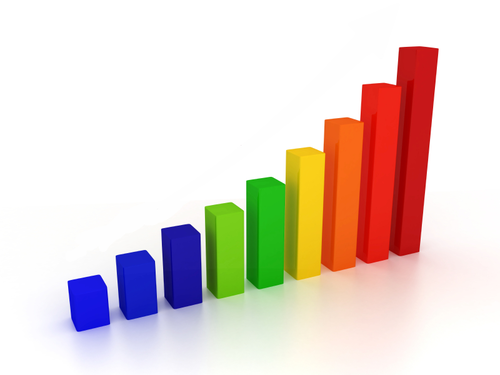
\includegraphics[width=0.5\textwidth]{matfmaster/img/graph.png}
  \caption{Графикон}
  \label{fig:grafikon}
\end{figure}

% primer jednostavnije matematičke formule
Ево и један пример математичке формуле: $e^{i\pi} + 1 = 0$. 
% primer referisanja na sliku
На слици \ref{fig:grafikon} приказан је један графикон.

% primer kompleksnije matematičke formule
$$
\int_a^b f(x)\ \mathrm{d}x \ =_{def}\ \lim_{\max{\Delta x_k \rightarrow 0}} \sum_{k=1}^n f(x_k^*)\Delta x_k
$$

% primer referisanja na poglavlja i strane poglavlja
Више детаља биће дато у глави \ref{chp:mikroservisi} на страни \pageref{chp:mikroservisi}.

% primer listinga koda

У тезу можемо убацити и програмски кôд.

\begin{verbatim}
Ovo je doslovni tekst.
\end{verbatim}

% \begin{english}
% \lstset{
%   language=C,
%   basicstyle=\ttfamily,
%   keywordstyle=\color{blue}
% }
% \begin{lstlisting}
% #include <stdio.h>

% int main() {
%   printf("Hello, world!\n");
%   return 0;
% }
% \end{lstlisting}
% \end{english}


Овај C програм се може превести помоћу преводиоца GCC.

% primer liste
Можемо правити и набрајања:
\begin{enumerate}
\item Анализа 1
\item Линеарна алгебра
\item Аналитичка геометрија
\item Основи програмирања
\end{enumerate}


% ------------------------------------------------------------------------------
\chapter{Микросервисна архитектура}
\label{chp:mikroservisi}
% ------------------------------------------------------------------------------

% Учестала унапређења технологија
% Учестало подизање (техничког и пословног) нивоа захтева
% инамичан пораст броја, сложености и величине софтверских пројеката.

Усложњавањем проблема који се решавају софтверским решењима расте и комплексност апликације која тај проблем решава. Као и многи комплексни математички проблеми, комплексност у софтверским решењима превазилази се разбијањем домена проблема у више поддомена. 

При коришћењу монолитне архитектуре проблем комплексности решења решава се техникама које теже ка што већој кохезивности кода. Кохезивност кода представља идеју груписања модула сличних функционалности заједно. 
Микросервисна архитектура такође почива на овом принципу, где је циљ комплетно раздвајање делова система уз јасно дефинисане границе. Микросервисна архитектура представља архитектурални стил који структуира систем као скуп малих сервиса који су минимално спрегнути, оријентисани ка специфичном домену, и лаки за интеграцију и одржавање. 



% Microservices - also known as the microservice architecture - is an architectural style that structures an application as a collection of services that are

% Highly maintainable and testable
% Loosely coupled
% Independently deployable
% Organized around business capabilities
% Owned by a small team
% The microservice architecture enables the rapid, frequent and reliable delivery of large, complex applications. It also enables an organization to evolve its technology stack.


Услед повећања нивоа захтева који се постављају при развоју софтвера, и учесталих унапређења технологија, 
за брзим развојем као и идејама које доноси агилни развој софтвера попут континуиране испоруке 

% ------------------------------------------------------------------------------
\chapter{Аутоматско тестирање софтвера}
\label{chp:testiranje}
% ------------------------------------------------------------------------------

% ------------------------------------------------------------------------------
\chapter{Имплементација и тестирање \textit{Gelos} апликације}
\label{chp:aplikacija}
% ------------------------------------------------------------------------------
Практични део рада представља имплементацију микросервисне апликације, као и система за тестирање те апликације. Циљ апликације је претраживање и помоћ при избору филма односно књиге за читање. Посебна пажња при изради апликације посвећена је системима за тестирање апликације како на јединичном, тако и на интеграционом и системском нивоу. Архитектурално решење за сваки део овог система је обрађен у склопу овог поглавља.

\section{Кратак преглед коришћених технологија}
\label{chp:tehnologije}

За израду микросервиса коришћен је развојни оквир \textit{Express.js} \cite{express} писан за извршно окружење \textit{Node.js} \cite{nodejs}. За складиштење података коришћен је систем за управљање базом података \textit{SQLite} \cite{sqlite} у комбинацији са алатом за објектно-релационо мапирање \textit{Sequelize} \cite{sequelize}. 

За израду клијентске апликације коришћенa jе библиотека \textit{React} \cite{react}. За стилизовање корисничког интерфејса коришћен развојни оквир \textit{Tailwind} \cite{tailwind}. 

За израду оквира за интеграционо и функционално тестирање система коришћен је развојни оквир \textit{Playwright} \cite{playwright} док је за генерисање лажних података за тестирање коришћена библиотека \textit{MSW} (енг. \textit{Mock Service Worker}) \cite{msw}. У склопу израде компонентних и јединичних тестова коришћена је библиотека \textit{React Testing Library} \cite{rtl} у комбинацији са \textit{Jest} \cite{jest} развојним оквиром.

\subsection{Окружење \textit{Node.js}}

\textit{Node.js} представља извршно окружење који омогућава извршавање \textit{JavaScript} кода ван оквира претраживача односно на самом северу. Могућност да се и клијентска и серверска страна апликације пишу истим програмским језиком и самим тим убрза процес развоја апликације, допринела је великој популарности језика.
Ипак, главну особину овог развојног оквира представља могућност да извршава неблокирајући, асинхрон к\^{o}д и тако елиминише потребу за чекањем  \cite{w3nodejs}.

У склопу овог пројекта коришћен је и \textit{npm} (енг. \textit{node package manager}) који омогућава једноставну контролу инсталација и верзија коришћених библиотека \cite{npm}. Како се пројекат састоји из више независних целина коришћена је "\textit{monorepo}" стратегија за контролу верзија. Ова стратегија омогућава да се из изворне датотеке покрећу различити делови система \cite{monorepo}.

\subsection{Развојни оквир \textit{Express.js}}

Инспирисан развојним оквиром \textit{Sinatra}, \textit{Express.js} се одликује својом једноставношћу, уз могућност да кроз различите библиотеке испуни специфичне захтеве апликације. \textit{Express.js} пружа минималан скуп функционалности које омогућавају једноставну обраду \textit{HTTP} захтева, рутирање и интеграцију са системом за управљање базама података \cite{express}. 

Како \textit{Express.js} представља веома ниску апстракцију \textit{HTTP} протокола, има врло добре перформансе, па је због те особине и своје једноставности постао стандардан алат за креирање веб сервера и програмских интерфејса апликације унутар \textit{Node.js }окружења \cite{mdnexpress}.

\subsection{Систем за управљање базама података \textit{SQLite} и \textit{Sequelize}}

\textit{SQLite} је систем за управљање базама података заснован на програмском језику \textit{C}. Дизајниран је тако да буде стабилан, брз и компатибилан са различитим платформама.  Насупрот другим \textit{SQL} системима за управљање базама података, нема засебан серверски процес већ компетну базу података чува унутар једне датотеке \cite{sqlite,sqlitetutorial}

Објектно-релационо мапирање представља технику која омогућава да се подацима из базе података приступа користећи парадигму објектно оријентисаног програмирања. Ова техника омогућава да се подацима приступа кроз објекте односно методе тих објеката па се компликовани \textit{SQL} упити апстрахују у интуитивне позиве функција. У потпуности се елиминише потреба за употребом \textit{SQL} језика па то додатно убрзава процес развоја софтвера \cite{orm}. \textit{Sequelize} је библиотека за објектно релационо мапирање која је базирана на технологији \textit{ Node.js} и подржава велики број система за управљање базама података попут \textit{Postgres, MySQL, MariaDB, Microsoft SQL Server и SQLite} \cite{sequelize}.

\subsection{\textit{React} библиотека}
\label{section:react}
\textit{React} библиотека представља једну од најпопуларнијих \textit{JavaScript} библиотека за израду корисничког интерфејса.  Почива на идеји да се свака апликација састоји од скупа компоненти које представљају енкапсулиране целине. Свака компонента представља вид шаблона па може употребити више пута са различитим параметрима што смањује редундатност написаног кода. Како су компоненте јединичне целине оне у себи садрже и приказ саме компоненте у виду \textit{HTML} елемената и \textit{CSS} правила, као и начин на који се те компоненте мењају, у виду \textit{JavaScript} кода \cite{react}.

\textit{React} прави виртуелно \textit{DOM} (енг. \textit{Document Object Model}) стабло које је ажурира право \textit{DOM} стабло само за компоненте које су промењене при некој акцији на корисничком интерфејсу. Ово омогућава да се промене дешавају брже и без ажурирања целе веб странице што омогућава креирање такозваних једностраничних апликација \cite{react}. 

Сама библиотека имплементира само основне функционалности потребне за креирање корисничког интерфејса док се за функционалности попут рутирања морају инсталирати додатне библиотеке. Једна од таквих је \textit{React router} библиотека која је коришћена у склопу овог пројекта \cite{reactRouter}.

\subsection{\textit{Tailwind} }

Стилизовање модерних веб страница које се приказују другачије у односу на величину екрана уређаја представља велики изазов у процесу развоја веб апликације. Појавом \textit{CSS} развојних оквира који садрже већ стилизоване шаблоне убрзао се развој апликација и омогућио да се и без много уложеног времена може имплементирати модеран кориснички интерфејс. Коришћењем већ постојећих шаблона губи се могућност за прављењем јединственог корисничког интерфејса па се и поред развојних оквира као што је \textit{Bootstrap} користе и стандардна \textit{CSS} правила \cite{bootstrap}.

\textit{Tailwind} представља \textit{CSS} развојни оквир који решава проблем на мање рестриктиван начин, задржава брзину и једноставност развоја коју пружају горе поменути развојни оквири, а дозвољава флексибилност коју пружа коришћење \textit{CSS} правила. То се постиже коришћењем предефинисаних класа које у себи садрже велики број функционалности које омогућавају кориснику да лако имплементира комплексне промене на корисничком интерфејсу \cite{tailwind}.


\subsection{\textit{Playwright}}

\textit{Playwright} је развојни оквир направљен за аутоматизацију системских (\textit{end to end}) тестова од стране \textit{Microsoft} тима. Оквир подржава више програмских језика као што су \textit{Јava}, \textit{Python}, \textit{C\#}  и \textit{JavaScript} \cite{playwright}.

Сваки претраживач садржи погонски део који је одговоран за трансформисање \textit{HTML} текста у веб страницу која се приказује на самом уређају. \textit{Playwright} користи протокол \textit{DevTools} који омогућава директну комуникацију са погонским делом претраживача у циљу извршавања тестова у претраживачу \cite{playwrightTutorial}. Ова особина чини оквир знатно бржим и стабилнијим од конкуретних технологија које користе протокол \textit{WebDriver}. \cite{playwrightVsSelenium,speedTest}. Оквир поджава извршавање на претраживачима као што су \textit{Chromium,  Firefox} и \textit{Webkit} \cite{playwright, chromium,webKit}.

Аутоматско чекање је једна од главних особина оквира. Пре сваке акције над елементом на веб страници, проверава се да ли је елемент видљив и активан па се тек онда наставља са извршавањем теста. Ово елиминише потребу за имплицитним чекањима у аутоматским тестовима. Имплицитна чекања, односно заустављање теста на предефинисан број секунди како би се одређен елемент учитао, представљају чест узрок нестабилних тестова. Аутоматско чекање такође смањује потребу за експлицитним чекањима, која заустављају тест док одређен услов није испуњен, јер се већина стандардно коришћених услова аутоматски проверава пред интеракцију са елементом. Смањен број експлицитних чекања у тесту доприноси томе да тест буде концизан и јасан.

Конкуретно извршавање тестова је подржано и једноставно се имплементира услед асинхроне природе \textit{Node.js} оквира. Оквир не подржава тестирање на реалним мобилним уређајима али подржава емулацију претраживача за мобилне телефоне.

Уз алате за тестирање корисничког интерфејса, \textit{Playwright} такође пружа алате за визуелно тестирање, компонентно тестирање, и тестирање програмских интерфејса апликације \cite{playwright}. Неки од тих алата биће приказани у даљем тексту.

\subsection{Библиотека за тестирање \textit{React} апликација и  \textit{Jest}}

Тестирање појединачних јединица и компоненти система који користи \textit{React} библиотеку може се постићи коришћењем библиотеке за тестирање \textit{React} апликација (енг. React testing library) \cite{rtl}. Библиотека омогућава тестирање појединачних чворова \textit{DOM} стабла из угла корисника. Свака \textit{React} компонента се претвара у \textit{DOM} чвор и помоћу \textit{JavaScript} библиотеке за тестирање - \textit{Jest}, проверавају се очекиване вредности унутар чвора. Ова библиотека пружа сигурност да се подаци приказују на очекиван начин без обзира на друге делове система, као и да различите јединице функционишу унутар компоненти којима припадају \cite{rtl,jest}

% Рећи после да не треба мешати тестирање React компоненти и компонентно тестирање....  


\subsection{Библиотека \textit{MSW}}

Како би тестови били поуздани и подаци који се користе унутар тестова морају бити поуздани. Такође потребно је тестирати клијентски део апликације независно од серверског дела. 

\textit{MSW} (енг. \textit{Mock Service Worker}) представља библиотеку која омогућава да се \textit{API} позиви који су упућени ка серверској страни апликације пресретну и уместо правих, клијентској апликацији врате предефинисани ,,лажни” одговори. Ово омогућава како тестирање клијентског дела апликације у изолацији, тако и могућност независног развоја клијентског и серверског дела апликације \cite{msw}. Да би одговарајући \textit{API} позиви били пресретнути потребно је дефинисати тачке јавног интерфејса и предефинисане податке који се шаљу клијентској страни апликације.

% ОВДЕ МОЖЕ СЛИКА MSW


\section{Архитектура и дизајн апликације}

Развијена апликација подељена је у две целине, на серверски и клијентски део. Серверски део апликације организован је у међусобно незавнисне микросервисе. Сваки микросервис има јасно дефинисан јавни интерфејс помоћу ког клијентска страна апликације приступа ресурсима и функционалностима које микросервис пружа. Подаци које микросервиси користе организовани су тако да сваки микросервис има своју базу података. Комуникација између микросервиса и клијентског дела апликације извршава се коришћењем \textit{HTTP} протокола. У наставку ове секције биће детаљније приказани имплементациони детаљи као и архитектурална решења за сваки од делова апликације.


\subsection{Микросервиси}

Серверски део апликације састоји се од два независна микросервиса \textit{Books} и \textit{Movies}. Архитектура коришћена при имплементацији оба микросервиса је \textit{МVC} (енг. \textit{Model View Controller}) па је структура пројекта подељена у одговарајуће целине:
\begin{enumerate}
\item Датотека \textit{index.js} --- покреће претходно дефинисан сервер на одговарајућем порту. Дефинисање јавног интерфејса микросервиса дешава се унутар датотеке \textit{server.js}
\item Рутери (у директоријуму \textit{routers}) --- повезују добијене \textit{HTTP} захтеве са компонентама које су одговорне за обраду тих захтева.
\item Контролери (у директоријуму \textit{controllers}) --- имплементирају бизнис логику микросервиса тако што обрађују захтеве и делегирају операције доменским моделима.
\item Описи и методе за иницијализацију модела (у директоријуму \textit{models}) ---  дефинишу поља модела и имплементирају методе које учитавају и парсирају податке из базе података.
\item Конфигурација  система за управљање базом података (у директоријуму \textit{services}) --- конфигурише објектно-релационо мапирање и путању до фајла у ком се налази база података.
\end{enumerate}

% Искористи после у првој секцији
% \footnote{Образац архитектуре Модел-Поглед-Контролер (енг. \textit{Model-View-Controller, MVC})
% се заснива на подели система на три целине, које имају различите функције. модел — представља структуру података, поглед — представља приказ података у корисничком окружењу, контролер — управљања подацима модела.}

\newpage
\subsubsection{Сервис \textit{Movies}}

Сервис \textit{Movies}, односно сервис филмова, је сервис задужен за управљање подацима о филмовима и оценама за те филмове. Доменски модел овог сервиса налази се на слици \ref{fig:moviesShema}. Ентитет \textit{Title} садржи податке о филму као што су име, година снимања, број минута и жанр филма, док ентитет \textit{Rating} садржи информације о просечној оцени као и о броју корисника који су дали оцену за филм на сајту \textit{IMDB}.

\begin{figure}[!ht]
  \centering
  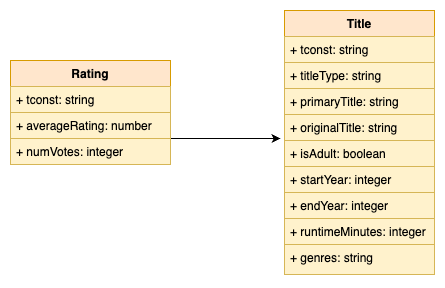
\includegraphics[width=0.75\textwidth]{matfmaster/img/moviesShema.png}
  \caption{Доменски модел сервиса \textit{Movies}}
  \label{fig:moviesShema}
\end{figure}
Сервис пружа јавни интерфејс помоћу ког је могуће добити информације о свим филмовима, о специфичном филму на основу његовог идентификатора као и добити листу филмова на основу упита. Детаљнији опис интерфејса приказан је у табели \ref{tbl:moviesAPI}.
\newpage
\begin{table}
\caption{Опис јавног интерфејса сервиса  \textit{Movies} }
\label{tbl:moviesAPI}
\begin{center}
\begin{tabular}{ |  p{0.3\linewidth} | p{0.3\linewidth}|  p{0.4\linewidth} | }
 
 \hline
  \textit{Опис} & \textit{Параметри} & \textit{Одговор при успешној обради} \\
  \hline
  \multicolumn{3}{|c|}{\textbf{GET api/v1/version}} \\
  \hline
  Дохватање актуелне верзије интерфејса
  & 
  
  & 
 version --- тренутна верзија интерфејса \\
  \hline
 \multicolumn{3}{|c|}{\textbf{GET api/v1/movies}} \\
  \hline
  Дохватање информација о свим доступним филмовима
  & 
  pagе --- број странице резултата (oпционо) \newline 
  size --- број филмова на страници (опционо)
  & 
  data --- објекат који садржи листу филмова са оценама \newline  
  meta --- објекат који саджи мета податке о листи \\
  \hline
   \multicolumn{3}{|c|}{\textbf{GET api/v1/movies/:id}} \\
  \hline
  Дохватање информација о специфичном филму 
  & 
  id --- идентификатор филма (обавезно)
  & 
  data --- објекат који садржи информације о специфичном филму\\
  \hline
   \multicolumn{3}{|c|}{\textbf{GET api/v1/movies/search}} \\
  \hline
  Претрага филмова на основу имена филма
  & 
  pagе --- број странице резултата (oпционо) \newline 
  size --- број филмова на страници (опционо) \newline 
  query --- кључна реч за претрагу (обавезно)
  & 
  data --- објекат који садржи листу филмова \newline  
  meta --- објекат који саджи мета податке о листи \\
   \hline
     \multicolumn{3}{|c|}{\textbf{GET api/v1/ratings}} \\
  \hline
 Дохватање свих оцена филмова
  & 
  pagе --- број странице резултата (oпционо) \newline 
  size --- број филмова на страници (опционо)
  & 
  data --- објекат који садржи листу o оцена филмова са њиховим насловом \newline 
  meta --- објекат који саджи мета податке о листи \\ 
  \hline
\end{tabular}
\end{center}
\end{table}

\newpage

\subsubsection{Сервис \textit{Books}}

Сервис Books, односно сервис књига је сервис задужен за управљање подацима о популарним књигама. Сервис омогућава претрагу популарних наслова, као и добијање информација о аутору, оцени наслова и других информација о књигама. Доменски модел овог сервиса налази се на слици \ref{fig:booksShema}. 
Сервис пружа програмски дефинисан интерфејс који омогућава излиставање целокупне листе књига које се налазе у бази података, као и претрагу по насловима.
\newpage

Сервис књига има врло сличан јавни интерфејс као и сервис филмова, али због разлика у доменима и количини података са којима располажу, овај сервис у склопу исте табеле садржи информације о књигама и инфомације о оценама тих књига. Детаљан опис функционалности које микросервис пружа може се видети у табели \ref{tbl:booksAPI}


\begin{table}
\caption{Опис јавног интерфејса сервиса \textit{Books}}
\label{tbl:booksAPI}
\begin{tabular}{ |  p{0.3\linewidth} | p{0.3\linewidth}|  p{0.4\linewidth} | }
\hline
\textit{Oпис} & \textit{Параметри} & \textit{Одговор при успешној обради} \\
\hline
\multicolumn{3}{|c|}{\textbf{GET api/v1/version}} \\
\hline
Дохватање актуелне верзије интерфејса & & 
version --- тренутна верзија интерфејса \\
\hline
\multicolumn{3}{|c|}{\textbf{GET api/v1/books/}} \\
\hline
Дохватање информација о свим доступним књигама & 
pagе --- број странице резултата (oпционо) \newline 
size --- број књига на страници (опционо)
& 
data --- објекат који садржи листу књига \newline
meta --- објекат који саджи мета податке о листи \\
\hline
\multicolumn{3}{|c|}{\textbf{GET api/v1/books/search}} \\
\hline
Претрага књига на основу наслова књиге &
pagе --- број странице резултата (oпционо) \newline 
size --- број књига на страници (опционо) \newline 
query --- кључна реч за претрагу (обавезно) 
  & 
data --- објекат који садржи листу књига \newline
meta --- објекат који саджи мета податке о листи \\
\hline
\end{tabular}
\end{table}


\begin{figure}[!ht]
  \centering
  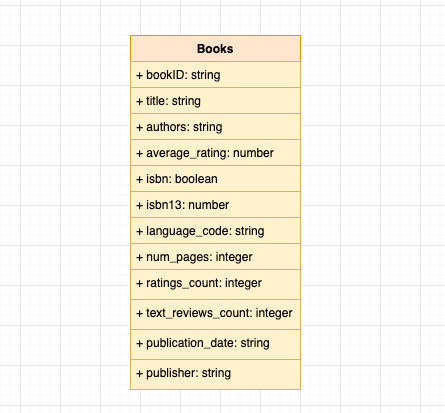
\includegraphics[width=0.5\textwidth]{matfmaster/img/booksShema.png}
  \caption{Доменски модел сервиса Books}
  \label{fig:booksShema}
\end{figure}
\newpage

\newpage


\subsection{Kлијентска апликација}

У склопу пројекта направљена је клијентска апликација која користи фукционалности које имплементирани микросервиси пружају. За имплементацију коришћена је библиотека \textit{React} као и помоћнa библиотекa \textit{React router} \cite{reactRouter}. Апликација је подељена на компоненте које представљају изоловане целине система и у себи садрже логику и визуелни приказ дела апликације. Појам \textit{React} компоненте детаљније је описан у секцији \ref{section:react}.

Централни део хијерархијске структуре апликације имплементиран је у компоненти \textit{Аpp}. Она сваку компоненту приказује унутар компоненте \textit{Layout} која дефинише распоред компоненти на страници, и изнад и испод сваке странице приказује компоненту \textit{Header} и \textit{Footer} респективно. \textit{Header} имплементира заглавље које садржи мени за навигацију, док \textit{Footer} представља подножје странице. Коришћењем библиотеке \textit{React router}, компонента \textit{App} приказује одговарајућу страницу у зависности од \textit{URL} путање. Уколико је путања неисправна биће приказана компонента \textit{Page404} која корисника обавештава о неисправно унешеној путањи.  

Странице представљају компоненте које интегришу више компоненти и имплементирају комуникацију са серверским делом апликације. Страница \textit{Homepage} представља полазну тачку клијентске апликације и садржи се од више презентационих картица које користе податке дефинисане у \textit{contents} директоријуму. Навигацијом кроз презентационe картицe или кроз горњи мени за навигацију корисник се преусмерава на неку од страница. 

Страница \textit{MoviesPage} омогућава кориснику презентацију као и претрагу оцењених филмова. Компонента  \textit{MoviesPage} користи јавни интерфејс \textit{Movies} сервиса и у складу са корисничким уносом података приказује листу филмова односно компоненти \textit{Movie}.  У склопу ове странице имплементирано је и приказивање вишестраничних резултата упита кроз компоненту \textit{Pagination}. Аналогно, страница \textit{BooksPage} приказује листу књига и омогућава претрагу књига по њиховом наслову користећи јавни интерфејс \textit{Books} сервиса. Обе компоненте користе компоненту \textit{SearchBar} која регулише унос наслова за претрагу. Празан унос у поље за претрагу кориснику враћа иницијалан скуп података.

Структура директоријума клијентске апликације осликава функционалност сваке од компоненти апликације. Компоненте које представљају странице апликације налазе се у директоријуму \textit{pages} док се компоненте које представљају делове страница налазе у директоријуму \textit{components}. Искључиво презентационе компоненте попут \textit{Loading} или \textit{Icons} компоненти налазе се у директоријуму \textit{ui}. Поред конфигурационих датотека у склопу апликације се налазе и систем за тестирање апликације као и систем за пресретање \textit{API} позива о којима ће бити речи у наредном поглављу.

% Можда нека слика апликације?







\section{Аутоматско тестирање апликације}


% ------------------------------------------------------------------------------
\chapter{Закључак}
% ------------------------------------------------------------------------------


% ------------------------------------------------------------------------------
% Literatura
% ------------------------------------------------------------------------------
\literatura

% ==============================================================================
% Završni deo teze i prilozi
\backmatter
% ==============================================================================

% ------------------------------------------------------------------------------
% Biografija kandidata
\begin{biografija}
\textbf{Вук Стефановић Караџић} (\emph{Тршић, 26. октобар/6. новембар
  1787. — Беч, 7. фебруар 1864.}) био је српски филолог, реформатор
српског језика, сакупљач народних умотворина и писац првог речника
српског језика.  Вук је најзначајнија личност српске књижевности прве
половине XIX века. Стекао је и неколико почасних доктората.
Учествовао је у Првом српском устанку као писар и чиновник у
Неготинској крајини, а након слома устанка преселио се у Беч,
1813. године. Ту је упознао Јернеја Копитара, цензора словенских
књига, на чији је подстицај кренуо у прикупљање српских народних
песама, реформу ћирилице и борбу за увођење народног језика у српску
књижевност. Вуковим реформама у српски језик је уведен фонетски
правопис, а српски језик је потиснуо славеносрпски језик који је у то
време био језик образованих људи. Тако се као најважније године Вукове
реформе истичу 1818., 1836., 1839., 1847. и 1852.
\end{biografija}
% ------------------------------------------------------------------------------

\end{document} 